% Section content template for individual Educative lessons
% This file contains the actual content for a specific section
% Generated from Educative API section content

% Section: Visualize Data in a Monitoring System
% Section ID: 5232629720285184
% Section Slug: visualize-data-in-a-monitoring-system
% Generated: 2025-12-07T18:38:35.103055

Large data centers have millions of servers, and visualizing the health data for all of them is challenging. An important aspect of monitoring a fleet of servers is to know which ones are alive and which ones are offline. A modern data center can house many thousands of servers in a building. We can use a heat map to display information about thousands of servers compactly in a data center.
\\
A \textbf{heat map} is a data visualization technique that shows the magnitude of a phenomenon in two dimensions by using colors.

\subsection{Using heat maps to troubleshoot}\label{S2f-QNTytrfgWQfixGTOB}
\\
We'll identify if a server is down by using heat maps. Each rack of servers is named and is sorted by data center, then cluster, then row, so problems common at any of these levels are readily apparent.
\\
A heat map depicting the operational state of a large number of components is an effective method. The health of each component is indicated by the color of each cell in a big matrix. Nodes with green cells operate within permitted parameters, while nodes with red cells are nonresponsive on multiple tries.
\\
Below, we have a heat map displaying the server's state.

\begin{figure}[htbp]
 \centering
 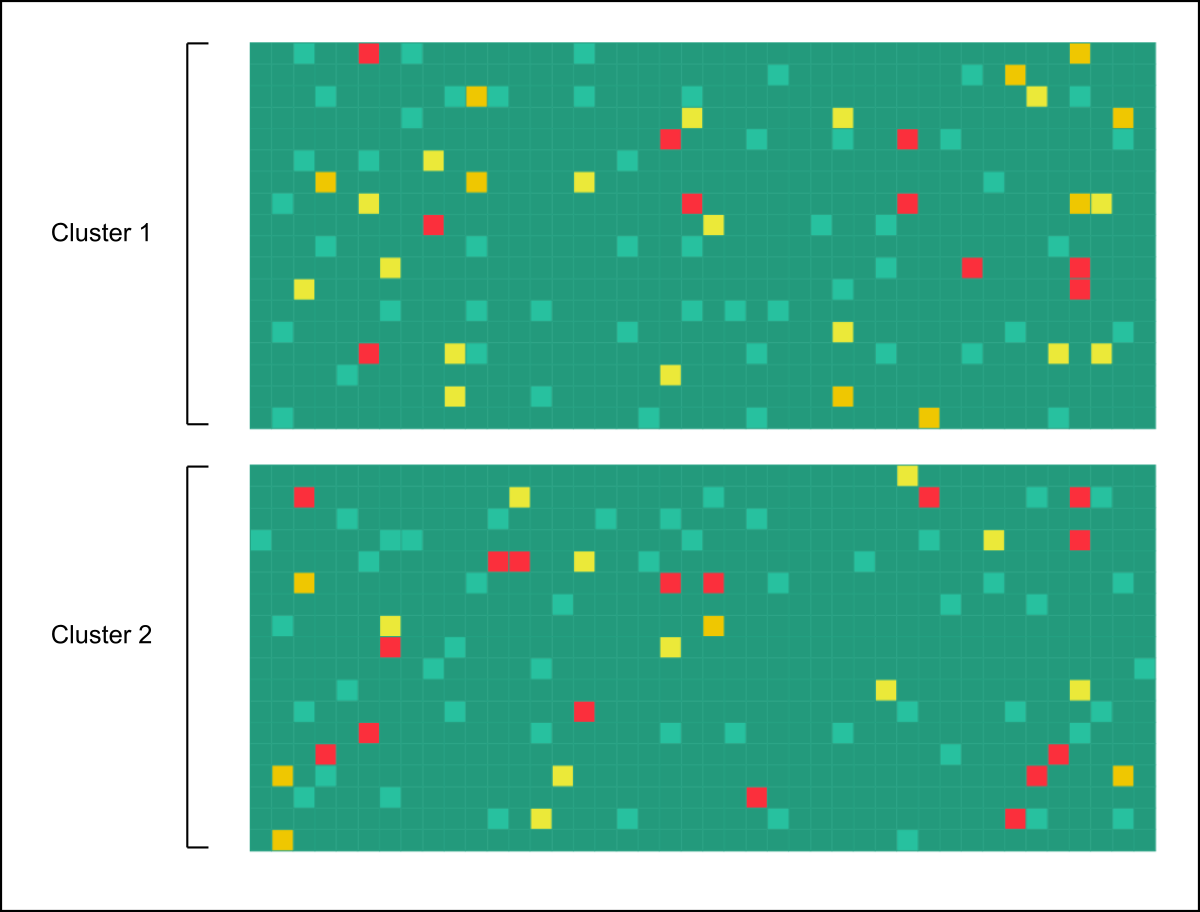
\includegraphics[width=0.5\textwidth]{Images/chapter_14/section_5232629720285184/6095589689655296.png}
 \caption{Viewing servers in a data center using heat maps}
\end{figure}

We can use heat maps for the globally distributed systems and continuously share the health information of a server. We can use one bit (one for live, zero for dead). For 1,000,000 servers, we have 125 KB of data. We can quickly find out which server is down by the red color and focus on the problematic parts.
\\
We can create similar heat maps to get a bird's-eye view of any resource, like filesystems, networking switches, links, and so on.
\\
Monitoring can be a tricky subject in system design interviews. Are you confident in what you've learned so far?
\\
Review these concepts using the widget below. Say ``Hello'' to Ed to get started.

\textit{Component type 'PromptAI' not yet supported.}

\subsection{Summary}\label{vVUdj_GnfgSDERL81TF1U}

\begin{itemize}
\item
\protect\phantomsection\label{OeDzDsb8_8I9VMNICwBji}
Monitoring systems are critical in distributed systems because they help in analyzing the system and alerting the stakeholders if a problem occurs.
\item
\protect\phantomsection\label{xh4QgPJQMuhfIDiGuDlXB}
We can make a monitoring system scalable using a hybrid of the push and pull methods.
\item
\protect\phantomsection\label{pHKTBrzYdeqyMuk56WqvV}
Heat maps are a powerful tool for visualization and help us learn about the health of thousands of servers in a compact space.
\end{itemize}

% End of section content